\section{Donut Delivery Experiment} \label{sec:exp_results}
An Amazon Mechanical Turk (AMT) experiment was designed in order to investigate how \xQ{} and \xO{} effect user behavior, if at all. In the experiment participants acted as `dispatch supervisors' of the UDT described in Sec.~\ref{sec:donut_delivery}.

\subsection{Method}
The key hypothesis was that users who were presented with self-confidence metrics would perform better in the dispatch task, and that this would result in a higher score.
The two \famsec{} metrics discussed herein (\xQ{} and \xO) were the experimental variables. Each was either `present' or `absent'. Therefore the experiment was a 2(\xQ) $\times$ 2(\xO) design, resulting in 4 conditions. Condition 1 was the `control' where both \xQ{} and \xO{} were absent. In condition 2 \xQ{} was present, in condition 3 \xO{} was present, and in condition 4 both \xQ{} and \xO{} were present. A screenshot of a typical task is shown in Fig.~\ref{fig:experiment_screenshot} (in the figure both \xQ{} and \xO{} are displayed indicating that this is condition 4, other conditions had an identical layout with the applicable values missing/present). Based on feedback from a pilot study the numerical values for \xQ{} and \xO{} were mapped to verbal descriptions ranging between `very bad' and `very good' to help users more easily grasp the scales when the two metrics were placed next to each other.

Participants were paid a base rate of $\$1.60$ for the Human Intelligence Task (HIT), and were able to get a bonus of up to $\$1.00$ based on their performance. Pilot data indicated that this would be equivalent to approximately \$7-10/hr. In practice the Turkers were quite a bit faster than those in the pilot study, and earned around \$13/hr. Source code for the experiment is available on Github\footnote{\url{https://github.com/COHRINT/SC_experiment}}

Generally, the responsibility of each participant was to decide whether the autonomous delivery vehicle should attempt to make a delivery, or decline the delivery. A successful delivery attempt resulted in $+1$ point, failure in $\-1$ point, and declining a delivery in $\-1/4$ point. After being trained (and passing a quiz) the participants saw a randomized sequence of 43 different delivery scenarios with varying maps. 

\subsection{Preliminary Results and Discussion}
Some preliminary data comparing the difference in cumulative `total score' is shown in Figure~\ref{fig:total_score}. The total number of participants represented here is N=255, with $n=\{63,63,64,65\}$ for conditions 1-4 respectively. Statistically the score for participants from each of conditions 2-4 have a significantly higher mean that of participants from condition 1 (i.e. $p<<0.01$ in all cases using and unequal variance T-test, see Fig.~\ref{fig:total_score}). This indicates that the participants were able to recognize limitations of the UDT and make more appropriate dispatch decisions. 

\begin{figure}[tbp]
    \centering
    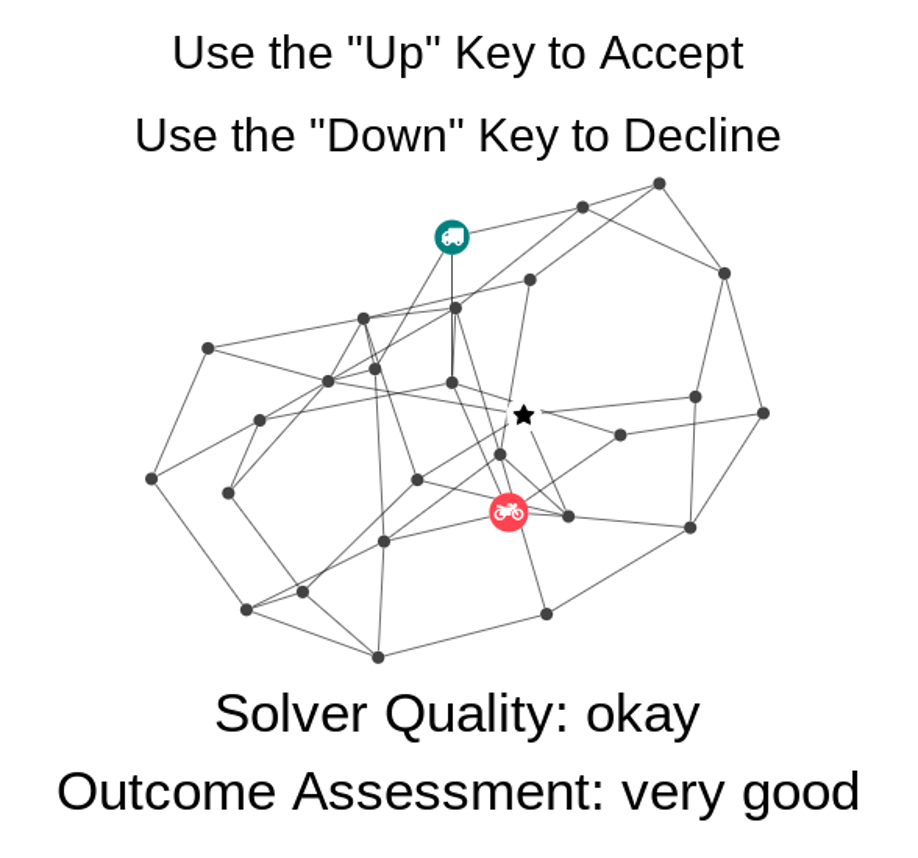
\includegraphics[width=0.45\linewidth]{Figures/experiment_screenshot_Compressed.png}
    \caption{Example screenshot from the Amazon Mechanical Turk experiment.} 
    \label{fig:experiment_screenshot}
\end{figure}

\begin{figure}[tbp]
    \centering
    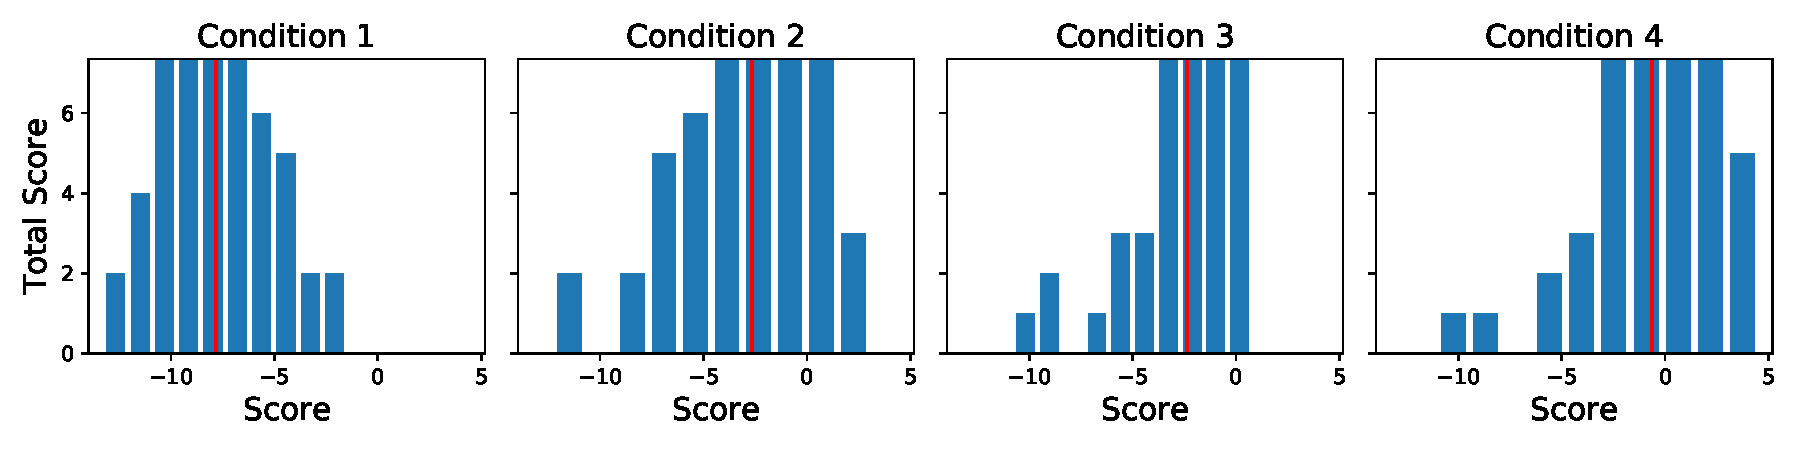
\includegraphics[width=1.0\linewidth]{Figures/total_score.pdf}
    \caption{Histogram of the Total Score from each condition. Red vertical lines indicate the sample mean. The p-value for the Unequal Variance T-Test (UT) with respect to condition 1 is shown in the legend of each plot.}
    \label{fig:total_score}
\end{figure}

At the end of the experiment participants answered survey questions about their perception of the UDT, how much they trusted the system, and how capable they thought it was. Our hypothesis is that the presence of self-confidence metrics would also affect these responses, but this data is still being analyzed.
